\subsection{第 18 课 | 排序算法}

\subsubsection{脑图}

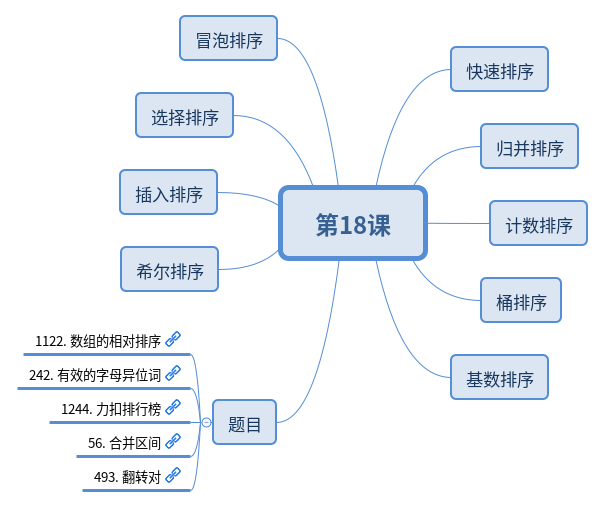
\includegraphics[width=100mm,height=86mm]{images/camp/第18课.png}

\subsubsection{题目}

\begin{itemize}
  \item \hyperref[leetcode:1122]{1122. 数组的相对排序}
  \item \hyperref[leetcode:242]{242. 有效的字母异位词}
  \item \hyperref[leetcode:1244]{1244. 力扣排行榜}
  \item \hyperref[leetcode:56]{56. 合并区间}
  \item \hyperref[leetcode:493]{493. 翻转对}
\end{itemize}

\subsubsection{扩展阅读}

\href{https://www.cnblogs.com/onepixel/p/7674659.html}{十大经典排序算法} \\
\href{https://www.bilibili.com/video/av25136272}{9 种经典排序算法可视化动画} \\
\href{https://www.bilibili.com/video/av63851336}{6 分钟看完 15 种排序算法动画展示}
